% !TEX program = pdflatex
\documentclass[12pt,a4paper]{article}

% =========================================================
% Encodage & langue
% =========================================================
\usepackage{needspace}
\usepackage{booktabs}
\usepackage{tabularx}

\newcommand{\NewMajorPart}{\clearpage}
\newcommand{\SubNeeds}[1]{\Needspace{#1\baselineskip}}

\newcommand{\roundedimg}[2][width=\textwidth]{%
  \sbox0{\includegraphics[#1]{#2}}%
  \begin{tikzpicture}
    \clip[rounded corners=10pt] (0,0) rectangle (\wd0,\ht0);
    \node[anchor=south west, inner sep=0pt] at (0,0) {\usebox0};
  \end{tikzpicture}%
}

\usepackage[T1]{fontenc}
\usepackage[utf8]{inputenc}
\usepackage[french]{babel}
\usepackage{longtable}
\usepackage{float}

% =========================================================
% Index
% =========================================================
\usepackage{makeidx}
\makeindex

% =========================================================
% Police
% =========================================================
\usepackage{helvet}
\renewcommand{\familydefault}{\sfdefault}

% =========================================================
% Paragraphes
% =========================================================
\setlength{\parindent}{1.25em}
\setlength{\parskip}{0pt}

% =========================================================
% Mise en page
% =========================================================
\usepackage{geometry}
\geometry{margin=2.5cm, headheight=14.5pt}
\usepackage{setspace}
\onehalfspacing

% =========================================================
% Listes
% =========================================================
\usepackage{enumitem}

\newlist{sq}{itemize}{1}
\setlist[sq]{%
  label=\rule{0.9ex}{0.9ex},
  leftmargin=3.2em,
  labelsep=0.35em,
  itemsep=0.1em,
  parsep=0pt,
  topsep=0.12em,
  partopsep=0pt
}

\newlist{num}{enumerate}{1}
\setlist[num]{%
  label=\textbf{[\arabic*]},
  leftmargin=3.2em,
  labelsep=0.35em,
  itemsep=0.1em,
  parsep=0pt,
  topsep=0.12em,
  partopsep=0pt
}

\setlist[itemize]{leftmargin=2.2em, itemsep=0.2em, topsep=0.2em}
\setlist[enumerate]{leftmargin=2.2em, itemsep=0.2em, topsep=0.2em}

% =========================================================
% Graphiques & en-têtes
% =========================================================
\usepackage{graphicx}
\usepackage{tikz}
\usepackage{xcolor}
\usepackage{colortbl}
\usepackage{fancyhdr}
\usepackage[hidelinks]{hyperref}
\usepackage{tcolorbox}
\tcbuselibrary{skins}
\usepackage{caption}
\captionsetup{font=small, labelfont=bf}

% =========================================================
% Styles de page
% =========================================================
\pagestyle{fancy}
\fancyhf{}
\lhead{\textbf{MEDISCAN AI}}
\rhead{\textbf{Rapport de Projet}}
\cfoot{\thepage}

\fancypagestyle{firstpage}{
  \fancyhf{}
  \cfoot{\thepage}
  \renewcommand{\headrulewidth}{0pt}
  \renewcommand{\footrulewidth}{0pt}
}

% =========================================================
% Macro
% =========================================================
\newcommand{\IntroPartie}[1]{%
\vspace{0.2cm}
\begin{center}
\textit{#1}
\end{center}
\vspace{0.3cm}
}

% =========================================================
% Titre
% =========================================================
\title{Rapport de Projet --- \textbf{MEDISCAN AI}\\[0.4em]
\large Plateforme de recherche multimodale d'images médicales par le contenu (\textbf{CBIR})}
\author{L3X1 --- Université Paris Cité}
\date{}

% =========================================================
\begin{document}
% =========================================================

% =========================================================
% PAGE DE GARDE
% =========================================================
\maketitle
\thispagestyle{firstpage}

\vspace{0.3cm}
\begin{center}
  
\includegraphics[width=0.5\textwidth]{assets/Logo.png}
\end{center}

\vspace{0.5cm}

\begin{center}
\textit{
Le présent document est le \textbf{rapport de projet} de \textbf{MEDISCAN AI},
prototype académique non clinique de recherche d'images médicales par le contenu.
Il couvre l'ensemble des travaux de l'équipe L3X1 : besoins, conception,
implémentation, tests et déploiement.
}
\end{center}

\vspace{0.8cm}

\section*{Informations document}
{\setlength{\parindent}{0pt}
\begin{tabularx}{\textwidth}{@{}lX@{}}
\textbf{Version :}         & v1.0 \\
\textbf{Référence :}       & Rapport de Projet MEDISCAN AI v1.0 \\
\textbf{Confidentialité :} & Interne projet (usage universitaire) \\
\textbf{Encadrant :}       & Camille Kurtz \\
\textbf{Équipe :}          & L3X1 (Taskin Ozan, Rayane Taouache, Ales Ferhani, Maxime Huang) \\
\end{tabularx}
}

% =========================================================
% ÉQUIPE
% =========================================================
\newpage
\section*{Équipe projet}
\addcontentsline{toc}{section}{Équipe projet}

\vspace{1.0cm}
L'équipe \textbf{L3X1} est composée de quatre étudiants de l'Université Paris Cité.
Chaque membre a contribué à plusieurs pôles en fonction de ses compétences.

\vspace{1.5cm}

\begin{center}
\begin{tabular}{cccc}
  \begin{tikzpicture}
    \clip (0,0) circle (1.2cm);
    \node at (0,0) {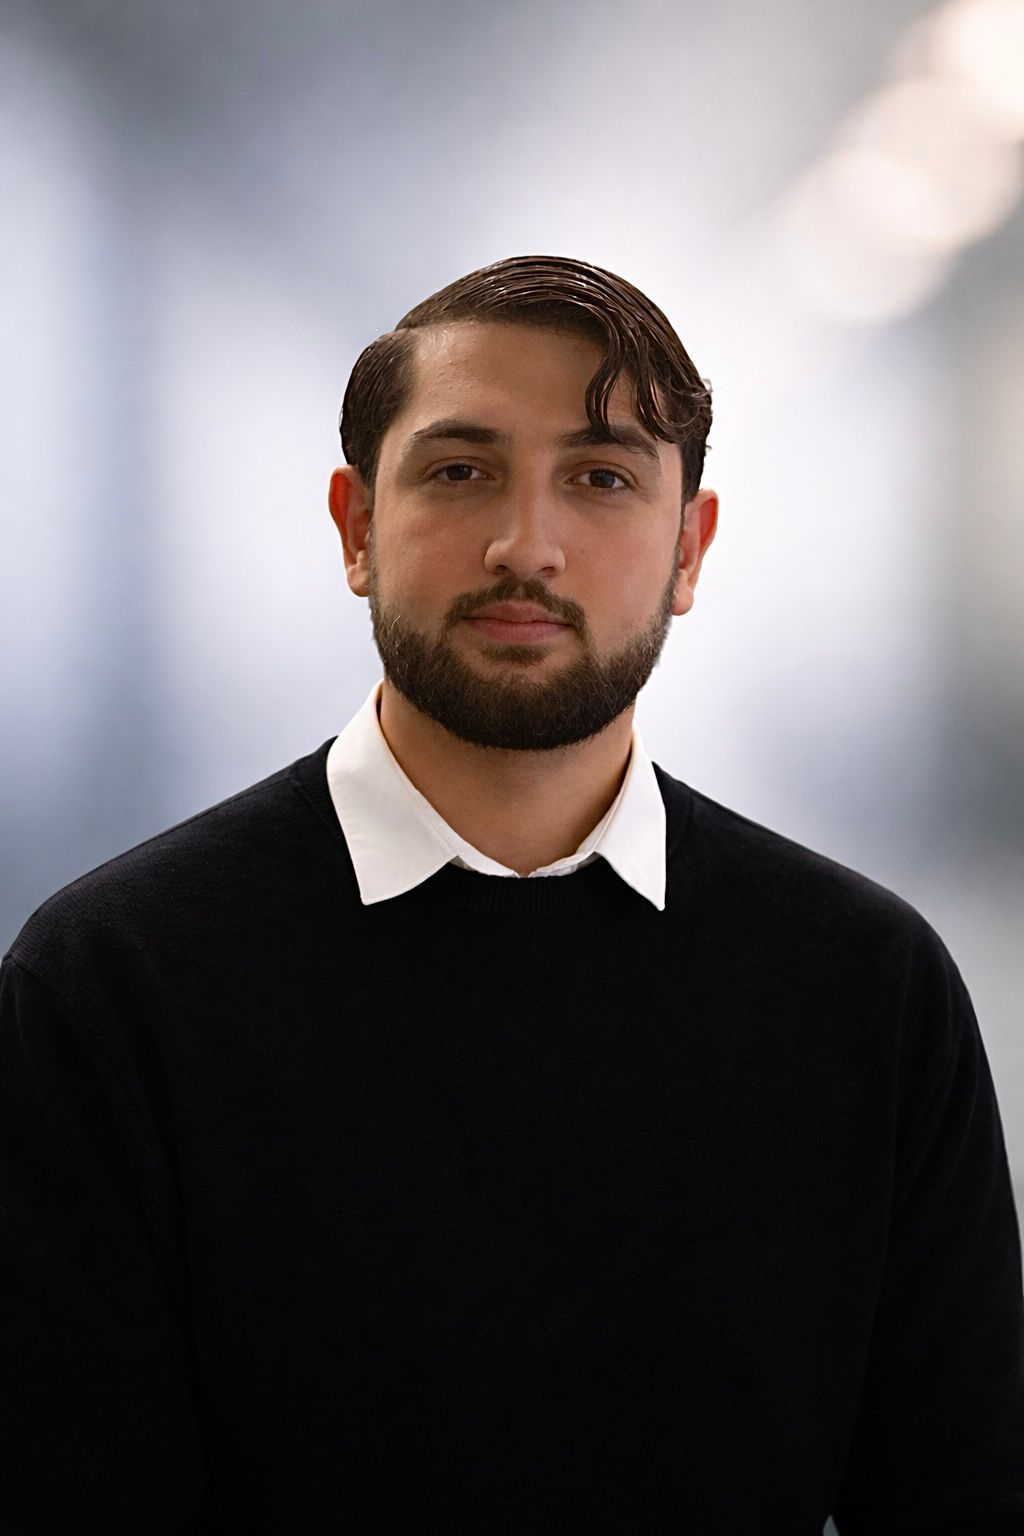
\includegraphics[width=2.4cm]{assets/photo-ozan.jpeg}};
  \end{tikzpicture}
  &
  \begin{tikzpicture}
    \clip (0,0) circle (1.2cm);
    \node at (0,0) {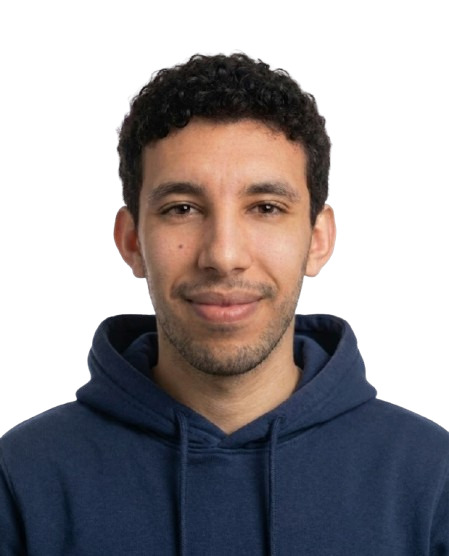
\includegraphics[width=2.4cm]{assets/photo-ales.jpeg}};
  \end{tikzpicture}
  &
  \begin{tikzpicture}
    \clip (0,0) circle (1.2cm);
    \node at (0,0) {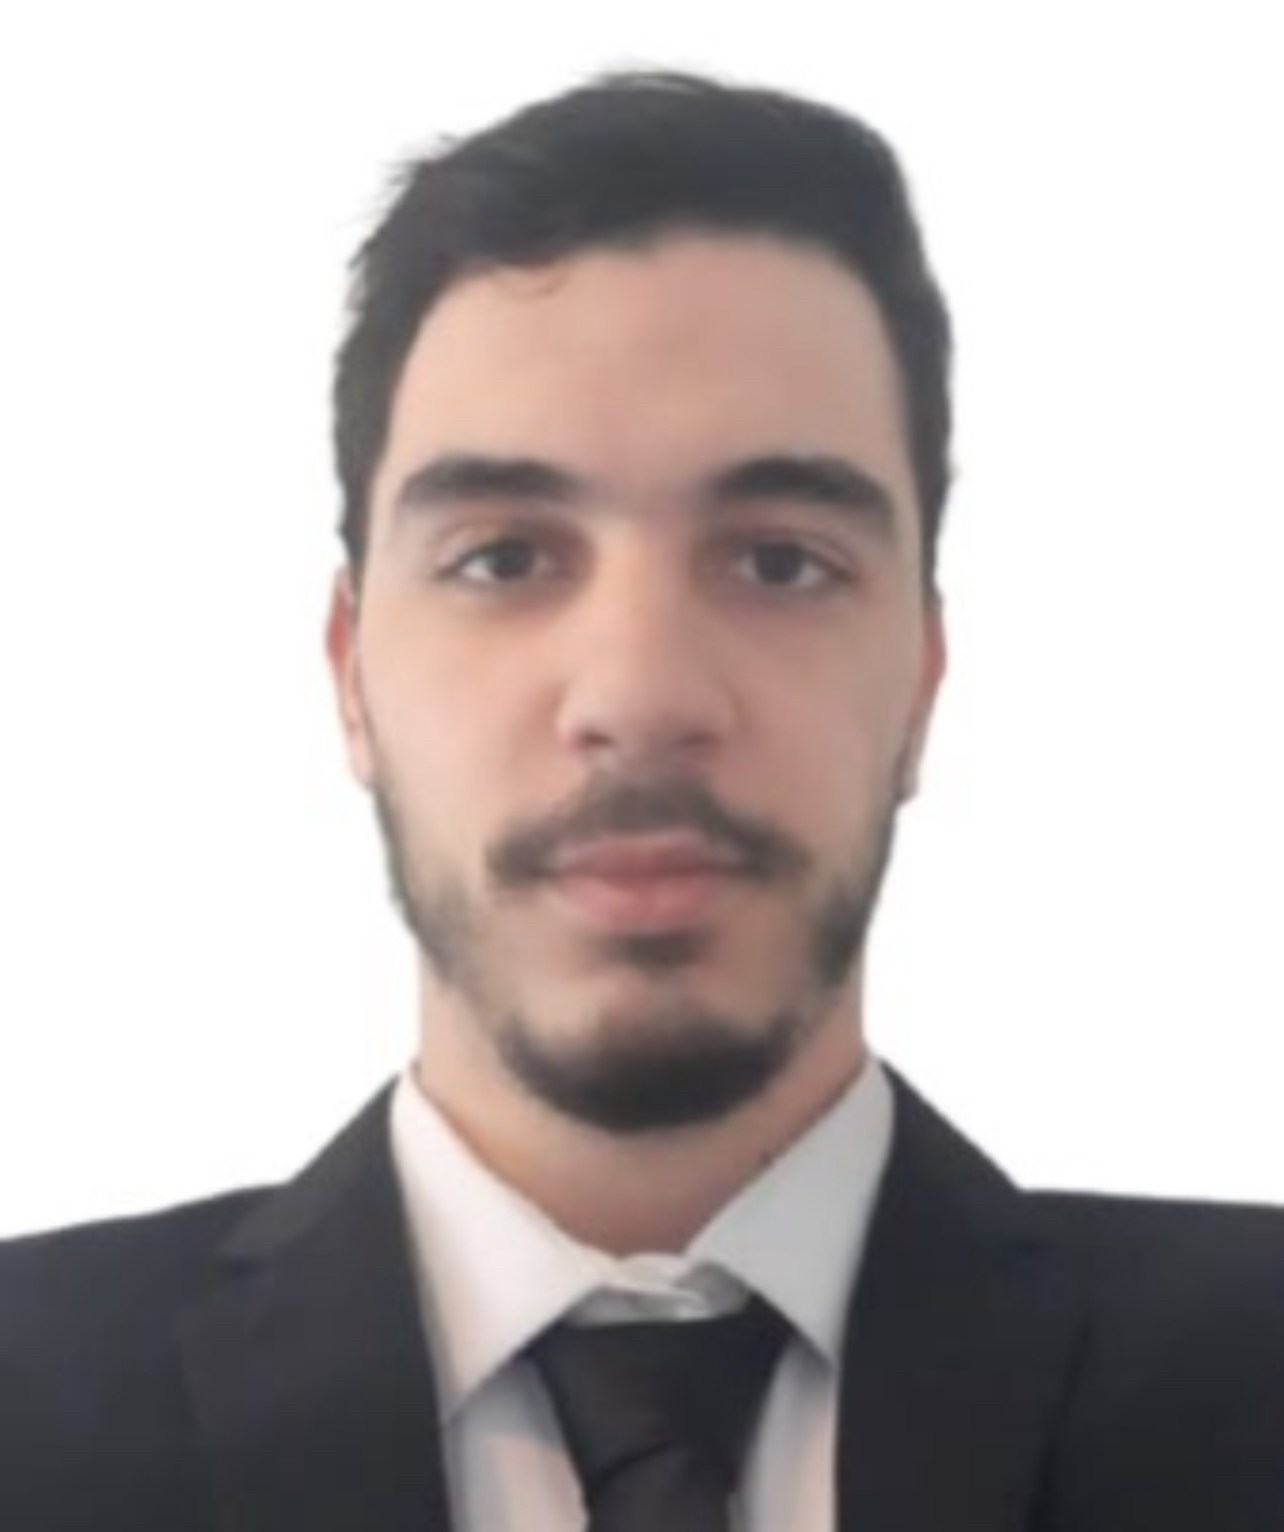
\includegraphics[width=2.4cm]{assets/photo-rayane.jpeg}};
  \end{tikzpicture}
  &
  \begin{tikzpicture}
    \clip (0,0) circle (1.2cm);
    \node at (0,0) {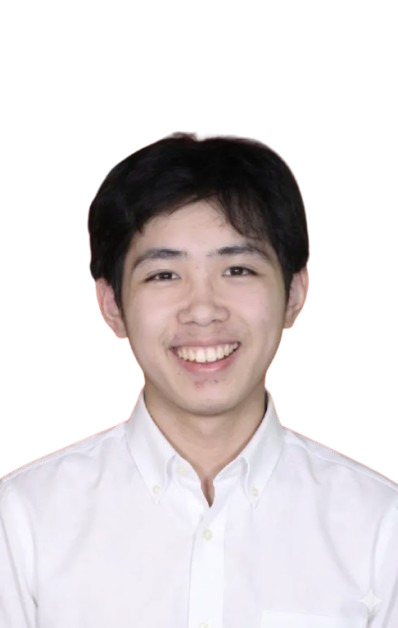
\includegraphics[width=2.4cm]{assets/photo-maxime.jpeg}};
  \end{tikzpicture}
  \\[0.4cm]
  \textbf{Taskin Ozan}
  & \textbf{Ferhani Ales}
  & \textbf{Taouache Rayane}
  & \textbf{Huang Maxime} \\[0.1cm]
  \textcolor[HTML]{1B3A6B}{\small AI / Frontend}
  & \textcolor[HTML]{1B3A6B}{\small AI / Test}
  & \textcolor[HTML]{1B3A6B}{\small Backend / Test}
  & \textcolor[HTML]{1B3A6B}{\small Frontend / Backend} \\
\end{tabular}
\end{center}

\vspace{1.5cm}

\begin{minipage}[t]{0.47\textwidth}
\begin{tcolorbox}[
  equal height group=team,
  colback=white, colframe=gray!50,
  boxrule=1pt, arc=5pt,
  left=8pt, right=8pt, top=8pt, bottom=8pt,
  borderline west={3pt}{0pt}{[HTML]{1E293B}}
]
{\small\textcolor[HTML]{64748B}{IA / Frontend}}\\[0.2cm]
\textbf{Taskin Ozan}\\[0.15cm]
{\small Architecture du système, pipeline CBIR,
fine-tuning BioMedCLIP, interface React.}
\end{tcolorbox}
\end{minipage}
\hfill
\begin{minipage}[t]{0.47\textwidth}
\begin{tcolorbox}[
  equal height group=team,
  colback=white, colframe=gray!50,
  boxrule=1pt, arc=5pt,
  left=8pt, right=8pt, top=8pt, bottom=8pt,
  borderline west={3pt}{0pt}{[HTML]{1E293B}}
]
{\small\textcolor[HTML]{64748B}{IA / Test}}\\[0.2cm]
\textbf{Ferhani Ales}\\[0.15cm]
{\small Scripts d'évaluation, stratégie de tests, traitement embeddings.}
\end{tcolorbox}
\end{minipage}

\vspace{1.2cm}

\begin{minipage}[t]{0.47\textwidth}
\begin{tcolorbox}[
  equal height group=team,
  colback=white, colframe=gray!50,
  boxrule=1pt, arc=5pt,
  left=8pt, right=8pt, top=8pt, bottom=8pt,
  borderline west={3pt}{0pt}{[HTML]{1E293B}}
]
{\small\textcolor[HTML]{64748B}{Backend / Test}}\\[0.2cm]
\textbf{Taouache Rayane}\\[0.15cm]
{\small API FastAPI, services backend, déploiement VPS, intégration MongoDB, tests d'intégration.}
\end{tcolorbox}
\end{minipage}
\hfill
\begin{minipage}[t]{0.47\textwidth}
\begin{tcolorbox}[
  equal height group=team,
  colback=white, colframe=gray!50,
  boxrule=1pt, arc=5pt,
  left=8pt, right=8pt, top=8pt, bottom=8pt,
  borderline west={3pt}{0pt}{[HTML]{1E293B}}
]
{\small\textcolor[HTML]{64748B}{Frontend / Backend}}\\[0.2cm]
\textbf{Huang Maxime}\\[0.15cm]
{\small Interface React, configuration Nginx, tests frontend.}
\end{tcolorbox}
\end{minipage}

\vspace{1.5cm}

\noindent Le projet a été développé \textbf{collectivement} : chaque membre a contribué
à l'ensemble des composants du système. Naturellement, au fil du projet, des expertises
se sont constituées au sein de l'équipe, reflétées dans la répartition des rôles ci-dessus.

% =========================================================
% SOMMAIRE
% =========================================================
\newpage
\tableofcontents

% =========================================================
% LISTE DES ILLUSTRATIONS
% =========================================================
\newpage
\listoffigures
\listoftables

% =========================================================
% GUIDE DE LECTURE
% =========================================================
\newpage
\section*{Guide de lecture}
\addcontentsline{toc}{section}{Guide de lecture}

\vspace{0.3cm}

Le présent \textbf{rapport de projet} documente l'intégralité du cycle de réalisation
de \textbf{MEDISCAN AI}. Il adopte une structure professionnelle couvrant la gestion
de projet, la conception, la réalisation et l'exploitation du système.

\vspace{0.6cm}

\textbf{Manager ou décideur - Vision stratégique}

\vspace{0.2cm}

Pour comprendre le projet et sa valeur ajoutée sans entrer dans les détails techniques :

\begin{sq}
  \item \textbf{Résumé exécutif} - synthèse du projet en une page
  \item \textbf{Chapitre 1} - contexte, enjeux métier et objectifs
  \item \textbf{Chapitre 9} - bilan, retour sur investissement et perspectives
\end{sq}

\vspace{0.6cm}

\textbf{Encadrant technique - Architecture et réalisation}

\vspace{0.2cm}

Pour évaluer les choix techniques et la qualité de l'implémentation :

\begin{sq}
  \item \textbf{Chapitre 2} - benchmark et justification des technologies retenues
  \item \textbf{Chapitre 5} - architecture globale, pipeline CBIR, modèle de données
  \item \textbf{Chapitre 6} - réalisation et extraits de code significatifs
  \item \textbf{Chapitre 8} - déploiement, configuration et maintenance
\end{sq}

\vspace{0.6cm}

\textbf{Encadrant pédagogique - Rigueur et méthode}

\vspace{0.2cm}

Pour évaluer la démarche projet et la conformité aux exigences :

\begin{sq}
  \item \textbf{Chapitre 3} - gestion de projet, méthodologie et planning
  \item \textbf{Chapitre 4} - cahier des charges, besoins fonctionnels et non fonctionnels
  \item \textbf{Chapitre 7} - recette, stratégie de tests et gestion des risques
\end{sq}

\vspace{0.6cm}

\textbf{Lecteur externe - Fonctionnalités et positionnement}

\vspace{0.2cm}

Pour comprendre ce que fait le système et comment il se positionne :

\begin{sq}
  \item \textbf{Chapitre 1} - contexte et enjeux
  \item \textbf{Chapitre 2} - benchmark et positionnement concurrentiel
  \item \textbf{Annexe C} - captures d'écran de l'application
\end{sq}

\vspace{0.6cm}

Le \textbf{glossaire} (Annexe F) définit les termes spécialisés du rapport.
Les \textbf{références} précisent les sources utilisées.
L'\textbf{index} (en fin de document) localise les mots-clés principaux.

% =========================================================
% RÉSUMÉ EXÉCUTIF
% =========================================================
\NewMajorPart
\section*{Résumé exécutif}
\addcontentsline{toc}{section}{Résumé exécutif}

\textbf{MEDISCAN AI} est une plateforme académique de recherche d'images médicales
par le contenu, réalisée par l'équipe L3X1 à l'Université Paris Cité.

\vspace{0.3cm}
\textbf{Contexte}

Les outils actuels reposent sur des mots-clés et ne permettent pas de retrouver
un cas similaire à partir d'une image médicale de référence.

\begin{sq}
  \item Les modèles d'IA récents rendent possible la recherche par similarité visuelle et sémantique.
  \item Aucune plateforme accessible ne combine ces deux approches sur images médicales
        tout en restant exécutable localement.
\end{sq}

\vspace{0.3cm}
\textbf{Solution}

L'équipe a conçu une plateforme \textbf{CBIR} multimodale sur trois modes :
\textbf{visuel} (DINOv2, 768D), \textbf{sémantique} (BioMedCLIP fine-tuné, 512D)
et \textbf{texte}. Une synthèse assistée par \textbf{LLM} complète les résultats.

\vspace{0.3cm}
\textbf{Architecture}

Le système est organisé en trois couches indépendantes.

\begin{sq}
  \item Backend \textbf{FastAPI}, neuf endpoints REST, index \textbf{FAISS} sur 80\,000 images,
        interface \textbf{React 19} et déploiement VPS avec \textbf{Nginx}.
\end{sq}

\vspace{0.3cm}
\textbf{Résultats}

Les évaluations menées sur \textbf{9\,140 requêtes} valident la pertinence du système
sur les trois modes.

\vspace{0.2cm}
{\setlength{\parindent}{0pt}
\begin{tabularx}{\textwidth}{@{}llXr@{}}
\toprule
\textbf{Mode} & \textbf{Modèle} & \textbf{Critère} & \textbf{Score} \\
\midrule
Visuel       & DINOv2      & Même modalité / anatomie / modalité+organe & 90,97 --- 88,58\,\% \\
Sémantique   & BioMedCLIP  & Même modalité / anatomie / modalité+organe & 91,29 --- 88,88\,\% \\
Texte        & BioMedCLIP  & Precision@10 (caption) / Top-1 hit        & 77,00 --- 100,00\,\% \\
\bottomrule
\end{tabularx}
}

\vspace{0.3cm}
\textbf{Cadre d'usage}

\textbf{MEDISCAN AI} est un prototype académique non clinique : il ne pose aucun diagnostic
et ne remplace pas un professionnel de santé.

\vspace{0.3cm}
\textbf{Perspectives}

\begin{sq}
  \item Intégration native du format \textbf{DICOM} et fine-tuning sur données internes.
  \item Mise en place d'un pipeline \textbf{CI/CD} pour automatiser les déploiements.
\end{sq}
% =========================================================
% CHAPITRE 1 — Contexte et enjeux
% =========================================================
\NewMajorPart
\section{Contexte et enjeux}

Cette section présente le cadre dans lequel s'inscrit \textbf{MEDISCAN AI},
la problématique qu'il adresse et les objectifs fixés à l'équipe.

\subsection{Contexte métier et motivation}

L'imagerie médicale produit des volumes croissants de données visuelles.
Les outils de recherche actuels reposent sur des mots-clés et des métadonnées textuelles.

\begin{sq}
  \item Un radiologue ne peut pas retrouver un cas similaire à partir d'une image de référence.
  \item Les modèles d'IA récents permettent de représenter une image sous forme de vecteur numérique.
  \item Cette représentation rend possible la recherche par similarité visuelle ou sémantique.
\end{sq}

\subsection{Problématique}

\begin{tcolorbox}[colback=gray!8, colframe=gray!40, boxrule=0.4pt, arc=2pt]
\textbf{\textit{Comment permettre à un professionnel de santé de retrouver des cas similaires
à partir d'une image médicale, de manière rapide, pertinente et respectueuse
de la confidentialité des données ?}}
\end{tcolorbox}

\subsection{Objectifs du projet}

L'objectif principal est de concevoir et réaliser une plateforme de recherche
multimodale d'images médicales par le contenu, exécutable localement.

\begin{sq}
  \item Proposer trois modes de recherche : visuel, sémantique et texte.
  \item Permettre la comparaison, le filtrage et la relance de recherche depuis les résultats.
  \item Générer une synthèse exploratoire assistée par LLM à partir des résultats.
\end{sq}

\subsection{Périmètre et limites}

Le système couvre la recherche par similarité sur un référentiel d'images indexées.

\begin{sq}
  \item \textbf{Inclus :} recherche visuelle et sémantique, interface web, API REST,
        déploiement local et VPS.
  \item \textbf{Exclus :} diagnostic médical, ingestion DICOM, certification clinique,
        données patient réelles.
\end{sq}

% =========================================================
% CHAPITRE 2 — Benchmark
% =========================================================
\NewMajorPart
\section{Benchmark et positionnement}

Cette section analyse les solutions existantes en recherche d'images médicales
et justifie les choix technologiques de \textbf{MEDISCAN AI}.

\subsection{Recherche d'images par le contenu (CBIR)}

Le CBIR désigne la recherche d'images par leur contenu visuel ou sémantique,
sans recours aux métadonnées textuelles.

\begin{sq}
  \item Les approches classiques (histogrammes, SIFT) sont peu robustes aux variations
        d'acquisition médicale.
  \item Les approches deep learning extraient des représentations vectorielles denses.
        Elles surpassent les approches classiques sur les tâches de similarité.
  \item En imagerie médicale, un modèle alignant image et langage est nécessaire
        pour capturer le sens clinique des images.
\end{sq}

\subsection{Solutions existantes et analyse comparative}

\begin{sq}
  \item \textbf{OpenI (NLM)} - indexe des rapports radiologiques mais repose
        uniquement sur la recherche textuelle, sans recherche par image.
  \item \textbf{MedGemma (Google DeepMind)} - modèle multimodal médical ouvert,
        orienté diagnostic et génération de texte, non recherche par similarité.
  \item \textbf{MedPaLM 2 (Google Health)} - grand modèle médical expert,
        sans recherche vectorielle ni interface de retrieval.
  \item \textbf{GPT-4o / Claude} - analyse d'images médicales possible,
        mais sans index ni recherche de cas similaires.
  \item \textbf{MONAI (NVIDIA)} - framework médical open source couvrant
        la segmentation et la classification, pas le CBIR interactif.
\end{sq}

\subsection{Positionnement de MEDISCAN AI}

Aucune solution existante ne combine les trois modes de recherche avec une exécution
locale et une interface produit complète.

\begin{sq}
  \item \textbf{MEDISCAN AI} propose la recherche par image, par texte et par similarité
        sémantique dans une même plateforme.
  \item L'exécution locale garantit la confidentialité : aucune image n'est transmise
        à un service externe.
\end{sq}

% =========================================================
% CHAPITRE 3 — Gestion de projet
% =========================================================
\NewMajorPart
\section{Gestion de projet}

Cette section présente la méthodologie de travail adoptée par l'équipe L3X1
et le planning du projet.

\vspace{0.4cm}

\subsection{Méthodologie}

\vspace{0.2cm}
L'équipe a adopté un cycle \textbf{incrémental} inspiré des méthodes agiles.

\vspace{0.2cm}
\begin{sq}
  \item \textbf{Incréments} - quatre livrables successifs : cœur CBIR, API backend,
        interface frontend, fine-tuning et évaluation.
  \item \textbf{Versionnement} - branches de fonctionnalité sur \textbf{GitHub},
        vérification avant chaque fusion sur la branche principale.
  \item \textbf{Coordination} - points de synchronisation bi-quotidiens sur \textbf{Discord}.
\end{sq}

\vspace{0.7cm}

\subsection{Planning et jalons}

\vspace{0.2cm}
Le projet s'est déroulé sur un semestre, structuré en quatre phases successives.

\vspace{0.2cm}
\begin{sq}
  \item \textbf{Phase 1} - analyse des besoins, choix techniques et mise en place
        de l'environnement de développement.
  \item \textbf{Phase 2} - implémentation du cœur CBIR : embedders, index FAISS,
        pipeline de recherche et API backend.
  \item \textbf{Phase 3} - développement de l'interface React, intégration
        frontend-backend et fine-tuning de BioMedCLIP sur ROCOv2.
  \item \textbf{Phase 4} - évaluation, tests, déploiement VPS et rédaction du rapport.
\end{sq}

\vspace{0.5cm}

\begin{figure}[H]
  \centering
  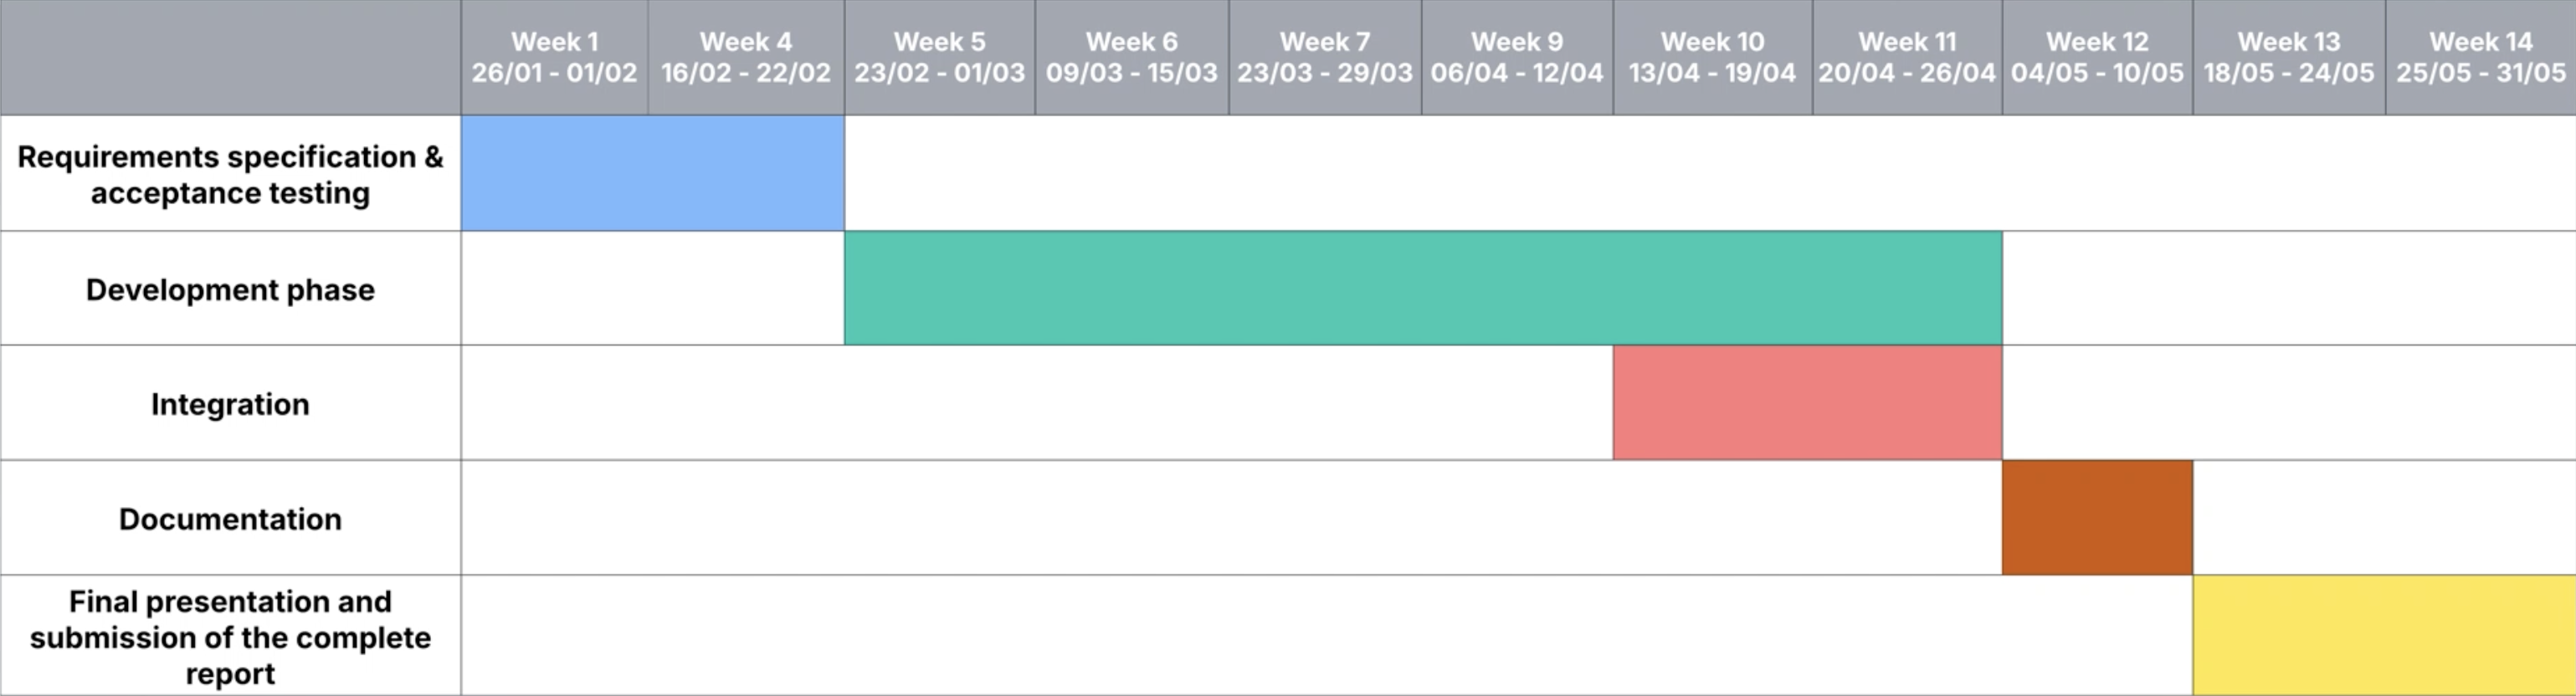
\includegraphics[width=\textwidth]{assets/gantt.png}
  \caption{Planning du projet MEDISCAN AI}
  \label{fig:gantt}
\end{figure}


% =========================================================
% CHAPITRE 4 — Cahier des charges
% =========================================================
\NewMajorPart
\section{Produit}

Cette section présente \textbf{MEDISCAN AI} en tant que produit :
son positionnement par rapport à la problématique, son ergonomie,
ses fonctionnalités et ses cas d'utilisation concrets.

\vspace{0.5cm}

\subsection{Réponse à la problématique}

\vspace{0.2cm}
\begin{tcolorbox}[colback=gray!8, colframe=gray!40, boxrule=0.4pt, arc=2pt]
\textbf{\textit{Comment permettre à un professionnel de santé de retrouver des cas similaires
à partir d'une image médicale, de manière rapide, pertinente et respectueuse
de la confidentialité des données ?}}
\end{tcolorbox}

\vspace{0.3cm}
\textbf{MEDISCAN AI} répond sur trois axes : \textbf{rapidité} (index FAISS, chargement lazy),
\textbf{pertinence} (trois modes de recherche) et \textbf{confidentialité} (exécution locale).

\vspace{0.3cm}

\begin{sq}
  \item \textbf{Utilisateurs cibles} : radiologues, chercheurs en imagerie médicale
        et étudiants en médecine.
  \item \textbf{Dataset} : 80\,000 images indexées issues du dataset public \textbf{ROCOv2}.
  \item \textbf{Langues} : interface disponible en français et en anglais.
\end{sq}

\vspace{0.7cm}

\subsection{Cas d'utilisation}

\vspace{0.2cm}
\textbf{MEDISCAN AI} comble un manque dans les outils disponibles : retrouver un cas
similaire à partir d'une image, sans mot-clé, directement par le contenu visuel ou clinique.

\vspace{0.3cm}
\begin{sq}
  \item \textbf{Radiologue} - retrouver rapidement des images morphologiquement proches
        d'un cas en cours d'analyse.
  \item \textbf{Chercheur} - explorer un corpus de 80\,000 images par similarité
        sémantique ou par requête textuelle.
  \item \textbf{Étudiant en médecine} - accéder à des cas comparables pour enrichir
        sa formation clinique.
\end{sq}

\vspace{0.3cm}
Le système s'exécute \textbf{localement} : aucune donnée n'est transmise à l'extérieur.
Il constitue un outil d'exploration et ne pose aucun diagnostic.

\vfill
\raggedright
\newpage
\subsection{Interface et ergonomie}

\begin{figure}[H]
  \centering
  \roundedimg[width=\textwidth]{assets/home.png}
  \caption{Page d'accueil de MEDISCAN AI}
  \label{fig:home}
\end{figure}

\vspace{0.6cm}

\noindent
\begin{minipage}[c]{0.28\textwidth}
  \roundedimg[width=\textwidth]{assets/theme-dark.png}
\end{minipage}
\hfill
\begin{minipage}[c]{0.67\textwidth}
  \captionsetup{justification=raggedright, singlelinecheck=false}
  \captionof{figure}{Sélecteur de thème et de langue}
  \vspace{0.2cm}
  {\small L'interface propose un \textbf{thème clair et sombre} adaptable
  à l'environnement de travail, ainsi qu'une bascule de langue
  \textbf{FR / EN} accessible depuis la barre de navigation.}
\end{minipage}

\vspace{0.6cm}

\noindent
\begin{minipage}[c]{0.28\textwidth}
  \parbox[c]{\textwidth}{%
  \setlength{\rightskip}{0pt}\setlength{\leftskip}{0pt}%
  \setlength{\parfillskip}{0pt plus 1fil}%
  {\small Le \textbf{hub central} permet de choisir entre les trois modes
  de recherche disponibles : Visual Search, Text Guided Search,
  et Interpretive Analysis.}\par}
\end{minipage}
\hfill
\begin{minipage}[c]{0.68\textwidth}
  \centering
  \roundedimg[width=\textwidth]{assets/hub.png}
  \captionsetup{justification=centering, singlelinecheck=false}
  \captionof{figure}{Hub de sélection du mode de recherche}
\end{minipage}

\newpage
\subsection{Modes de recherche}

\vspace*{0.5cm}
\noindent L'application propose trois modes complémentaires accessibles depuis le hub central.

\vspace{0.8cm}
\noindent
\begin{minipage}[c]{0.65\textwidth}
  \centering
  \roundedimg[width=\textwidth]{assets/visual-analysis.png}
  \captionsetup{justification=centering, singlelinecheck=false}
  \captionof{figure}{Mode Visual Analysis}
\end{minipage}
\hfill
\begin{minipage}[c]{0.31\textwidth}
  \raggedright
  {\small L'utilisateur dépose une image médicale.
  Le système retourne les images visuellement proches
  via \textbf{DINOv2} (768D).
  Adapté à la recherche par morphologie et structure anatomique.}
\end{minipage}

\vspace{1.4cm}

\noindent
\begin{minipage}[c]{0.31\textwidth}
  \raggedright
  {\small Recherche par proximité médicale via \textbf{BioMedCLIP} fine-tuné (512D).
  Privilégie le sens clinique sur la ressemblance visuelle.}
\end{minipage}
\hfill
\begin{minipage}[c]{0.65\textwidth}
  \centering
  \roundedimg[width=\textwidth]{assets/interpretive-analysis.png}
  \captionsetup{justification=centering, singlelinecheck=false}
  \captionof{figure}{Mode Interpretive Analysis}
\end{minipage}

\vspace{1.4cm}

\noindent
\begin{minipage}[c]{0.65\textwidth}
  \centering
  \roundedimg[width=\textwidth]{assets/text-query.png}
  \captionsetup{justification=centering, singlelinecheck=false}
  \captionof{figure}{Mode Text Query}
\end{minipage}
\hfill
\begin{minipage}[c]{0.31\textwidth}
  \raggedright
  {\small L'utilisateur saisit une description clinique.
  Le système retourne les images alignées
  via \textbf{BioMedCLIP} (500 caractères max).}
\end{minipage}

\subsection{Résultats et exploration}

\vspace{0.2cm}
\noindent Une fois la recherche lancée, l'interface propose des outils d'exploration
et de relance pour affiner les résultats.

\vfill
\begin{center}
  \roundedimg[width=0.85\textwidth]{assets/result-filter.png}
\end{center}
\captionsetup{justification=centering, singlelinecheck=false}
\captionof{figure}{Grille de résultats avec filtres et scores de similarité}
\vspace{0.15cm}
\noindent{\small Les filtres affinent les résultats sans relancer la recherche :
\textbf{score}, \textbf{caption}, \textbf{CUI} et \textbf{tri}.}
\vspace{0.9cm}
\vfill
\noindent
\begin{minipage}[c]{0.62\textwidth}
  \centering
  \roundedimg[width=\textwidth]{assets/relance.png}
  \captionsetup{justification=centering, singlelinecheck=false}
  \captionof{figure}{Relance de recherche depuis une sélection d'images}
\end{minipage}
\hfill
\begin{minipage}[c]{0.34\textwidth}
  \raggedright
  {\small Une sélection d'images devient une nouvelle requête via centroïde d'embeddings.
  \begin{num}
    \item Sélectionner une ou plusieurs images.
    \item Relancer depuis la sélection.
  \end{num}}
\end{minipage}
\vfill

\vspace*{1.2cm}
\begin{center}
  \roundedimg[width=0.85\textwidth]{assets/comparaison.png}
\end{center}
\captionsetup{justification=centering, singlelinecheck=false}
\captionof{figure}{Comparaison entre l'image requête et les résultats retournés}
\vspace{0.2cm}
\noindent{\small L'interface affiche côte à côte l'image requête et les résultats retournés,
permettant une comparaison visuelle directe.}

\vspace{1.2cm}
\vfill
\noindent
\begin{minipage}[c]{0.34\textwidth}
  \raggedright
  {\small Le module de synthèse analyse les résultats et génère
  une interprétation exploratoire assistée par IA.}
  \vspace{0.3cm}
  {\small
  \begin{num}
    \item Synthèse générée via \textbf{Groq} à partir des captions des résultats.
    \item Identifie les patterns récurrents sans poser de diagnostic.
  \end{num}}
\end{minipage}
\hfill
\begin{minipage}[c]{0.62\textwidth}
  \centering
  \roundedimg[width=\textwidth]{assets/ai_summary.png}
  \captionsetup{justification=centering, singlelinecheck=false}
  \captionof{figure}{Synthèse exploratoire générée par IA}
\end{minipage}
\vfill

% =========================================================
% CHAPITRE 5 — Technologies clés
% =========================================================
\NewMajorPart
\section{Technologies clés}

% =========================================================
% CHAPITRE 6 — Déploiement et exploitation
% =========================================================
\NewMajorPart
\section{Déploiement et exploitation}

\vspace{0.2cm}
Cette section présente l'infrastructure mise en place pour rendre \textbf{MEDISCAN AI}
accessible en production, ainsi que les choix garantissant sa stabilité et son évolutivité.

\subsection{Architecture et pipeline de déploiement}

\vspace{0.2cm}
L'application est déployée sur un \textbf{VPS Hostinger},
accessible via \texttt{mediscan-ai.site}.

\begin{sq}
  \item \textbf{Nginx} - reverse proxy, routage des requêtes frontend et backend.
  \item \textbf{Gunicorn + Uvicorn} - serveur ASGI pour l'API FastAPI.
  \item \textbf{systemd} - gestion des services et redémarrage automatique.
\end{sq}

\vspace{0.2cm}
Le déploiement suit un pipeline en quatre étapes.

\begin{num}
  \item Configuration du serveur Linux : mises à jour, firewall, ports 80/443.
  \item Installation des dépendances backend et build du frontend (Vite).
  \item Configuration Nginx avec virtual host et certificat SSL.
  \item Activation des services systemd pour le backend et le frontend.
\end{num}

\subsection{Production, accessibilité et évolutivité}

\vspace{0.2cm}
\textbf{MEDISCAN AI} est déployé en production et utilisable depuis n'importe quel navigateur,
sans installation côté utilisateur.

\begin{sq}
  \item \textbf{Accessibilité} - le service est disponible 24h/24 via
        \texttt{mediscan-ai.site}, avec connexion chiffrée HTTPS.
  \item \textbf{Confidentialité} - aucune image n'est transmise à un service externe ;
        tout le traitement s'effectue sur le serveur de l'équipe.
  \item \textbf{Stabilité} - le redémarrage automatique (systemd) garantit
        la continuité du service en cas d'arrêt inattendu.
\end{sq}

\vspace{0.2cm}
L'architecture choisie permet une montée en charge progressive.

\begin{sq}
  \item L'index FAISS est conçu pour passer de 80\,000 à plusieurs millions d'images
        sans modifier l'interface ni l'API.
  \item Le backend FastAPI est sans état (\textit{stateless}) : plusieurs instances
        peuvent être déployées en parallèle derrière Nginx pour absorber la charge.
  \item L'ajout d'un nouveau mode de recherche ou d'un nouveau modèle d'embedding
        ne nécessite pas de refonte de l'architecture.
\end{sq}

% =========================================================
% CHAPITRE 7 — Évaluation et résultats
% =========================================================
\NewMajorPart
\section{Évaluation et résultats}

% =========================================================
% CHAPITRE 8 — Difficultés rencontrées
% =========================================================
\NewMajorPart
\section{Difficultés rencontrées}

% =========================================================
% CHAPITRE 9 — Bilan et retour d'expérience
% =========================================================
\NewMajorPart
\section{Bilan et retour d'expérience}

% =========================================================
% CHAPITRE 10 — Perspectives
% =========================================================
\NewMajorPart
\section{Perspectives}

% =========================================================
% RÉFÉRENCES BIBLIOGRAPHIQUES
% =========================================================
\NewMajorPart
\section*{Références bibliographiques}
\addcontentsline{toc}{section}{Références bibliographiques}

\begin{num}
  \item M.~Caron \textit{et al.}, ``Emerging Properties in Self-Supervised Vision
        Transformers,'' \textit{ICCV}, 2021.
  \item S.~Zhang \textit{et al.}, ``BioMedCLIP: a multimodal biomedical foundation
        model,'' \textit{arXiv:2303.00915}, 2023.
  \item J.~Johnson, M.~Douze, H.~Jégou, ``Billion-scale similarity search with GPUs,''
        \textit{IEEE Transactions on Big Data}, 2019.
  \item FastAPI Documentation. \url{https://fastapi.tiangolo.com}
  \item React Documentation. \url{https://react.dev}
\end{num}

% =========================================================
% ANNEXES
% =========================================================
\NewMajorPart
\appendix

\section{Guide d'installation et de déploiement}

\subsection*{Prérequis}

\begin{sq}
  \item Python 3.11+, Node.js 20+, Git.
  \item 4 Go de RAM minimum (index FAISS + modèles chargés en mémoire).
  \item Clé API Groq pour la synthèse IA.
\end{sq}

\subsection*{Installation backend}

\begin{num}
  \item Cloner le dépôt : \texttt{git clone <url> \&\& cd mediscan-cbir}
  \item Créer l'environnement virtuel : \texttt{python -m venv .venv \&\& source .venv/bin/activate}
  \item Installer les dépendances : \texttt{pip install -r requirements.txt}
  \item Copier le fichier de configuration : \texttt{cp .env.example .env}
        puis renseigner la clé API Groq et les chemins des index.
  \item Lancer le serveur : \texttt{uvicorn main:app -{}-host 0.0.0.0 -{}-port 8000}
\end{num}

\subsection*{Installation frontend}

\begin{num}
  \item Aller dans le répertoire frontend : \texttt{cd frontend}
  \item Installer les dépendances : \texttt{npm install}
  \item Lancer en développement : \texttt{npm run dev}
  \item Ou compiler pour la production : \texttt{npm run build}
\end{num}

\subsection*{Déploiement VPS (production)}

\begin{sq}
  \item Configurer Nginx comme reverse proxy vers \texttt{localhost:8000} (backend)
        et le dossier \texttt{dist/} (frontend).
  \item Créer un service \textbf{systemd} pour Gunicorn et l'activer
        avec \texttt{systemctl enable mediscan}.
  \item Configurer le certificat SSL avec Certbot pour le domaine \texttt{mediscan-ai.site}.
\end{sq}

\section{Documentation API REST}

Les neuf endpoints de l'API sont exposés sous la base \texttt{/api/v1}.

\vspace{0.3cm}
{\setlength{\parindent}{0pt}
\begin{tabularx}{\textwidth}{@{}llX@{}}
\toprule
\textbf{Méthode} & \textbf{Endpoint} & \textbf{Description} \\
\midrule
POST & \texttt{/search/visual}    & Recherche visuelle par image (DINOv2). \\
POST & \texttt{/search/semantic}  & Recherche sémantique par image (BioMedCLIP). \\
POST & \texttt{/search/text}      & Recherche par description textuelle (BioMedCLIP). \\
POST & \texttt{/search/multisel}  & Relance depuis une sélection d'images (centroïde). \\
GET  & \texttt{/synthesis}        & Génère la synthèse IA pour un ensemble de résultats. \\
GET  & \texttt{/export/json}      & Export des résultats au format JSON. \\
GET  & \texttt{/export/csv}       & Export des résultats au format CSV. \\
GET  & \texttt{/export/pdf}       & Export des résultats au format PDF. \\
GET  & \texttt{/health}           & Vérification de l'état du service. \\
\bottomrule
\end{tabularx}
}

\section{Captures d'écran de l'application}

\section{Extraits de code complets}

\section{Résultats de tests détaillés}

\section{Glossaire}

\begin{description}[leftmargin=7em, style=sameline]
  \item[CBIR]       \textit{Content-Based Image Retrieval} --- recherche d'images
                    par le contenu visuel ou sémantique, sans recours à des métadonnées
                    textuelles manuelles.
  \item[Embedding]  Représentation vectorielle d'une image ou d'un texte dans un espace
                    de grande dimension, calculée par un réseau de neurones.
  \item[FAISS]      \textit{Facebook AI Similarity Search} --- bibliothèque de recherche
                    de voisins les plus proches dans des espaces vectoriels de grande dimension.
  \item[DINOv2]     Modèle de vision auto-supervisé développé par Meta AI, utilisé pour
                    extraire des représentations visuelles de dimension 768.
  \item[BioMedCLIP] Modèle multimodal pré-entraîné sur des données biomédicales, alignant
                    images et textes dans un espace vectoriel commun de dimension 512.
  \item[Fine-tuning] Adaptation d'un modèle pré-entraîné à un domaine spécifique par un
                    entraînement complémentaire sur des données ciblées.
  \item[Top-k]      Les $k$ résultats les plus similaires à une requête, retournés par
                    ordre décroissant de similarité.
  \item[LLM]        \textit{Large Language Model} --- modèle de langage de grande taille,
                    utilisé ici pour générer une synthèse exploratoire à partir des résultats.
  \item[Groq]       Service d'inférence LLM rapide, utilisé pour la génération de la
                    synthèse assistée.
  \item[ROCOv2]     \textit{Radiology Objects in Context v2} --- dataset public d'images
                    médicales annotées avec des captions et des concepts UMLS (CUI).
  \item[CUI]        \textit{Concept Unique Identifier} --- identifiant unique d'un concept
                    dans la nomenclature médicale UMLS.
  \item[UMLS]       \textit{Unified Medical Language System} --- système de terminologie
                    médicale unifié, référence pour les concepts cliniques.
  \item[FastAPI]    Framework Python asynchrone pour la création d'API REST, utilisé comme
                    couche applicative backend du système.
  \item[React]      Bibliothèque JavaScript pour la construction d'interfaces utilisateur,
                    utilisée pour le frontend du système.
  \item[Vite]       Outil de build et de développement frontend rapide, utilisé pour
                    compiler et servir l'application React.
  \item[MongoDB]    Base de données orientée documents, utilisée pour l'enrichissement
                    optionnel des métadonnées associées aux résultats de recherche.
  \item[Centroïde]  Vecteur moyen de plusieurs embeddings, utilisé pour la relance
                    multi-sélection afin de représenter la tendance commune d'un groupe.
\end{description}

% =========================================================
% INDEX
% =========================================================
\NewMajorPart
\printindex

% =========================================================
\end{document}
% =========================================================